\chapter{控制系统的数学模型}
\section{建立数学模型的方法}
我们通过一下的几种方法建立系统的数学模型：
\begin{enumerate}
    \item 机理分析法(\textbf{白箱模型}):
        根据基本的物理规律、化学规律以及能量守恒定律等，动态系统可以用微分方程描述
    \item 试验法/测试法(\textbf{黑箱模型})：
        通过一些经典信号激励，看系统的响应如何（脉冲响应，阶跃响应.....）
    \item 综合法(\textbf{灰箱模型})：
        一般通过机理分析建立模型的结构，然后通过系统辨识确定模型参数
\end{enumerate}

\section{物理系统的数学模型举例}
\begin{example}
    如图所示为弹簧-质量块-阻尼系统，设外界输入为$F$，滑块输出量为$y$和$v$，则可以列出以下式子：
    \begin{center}
        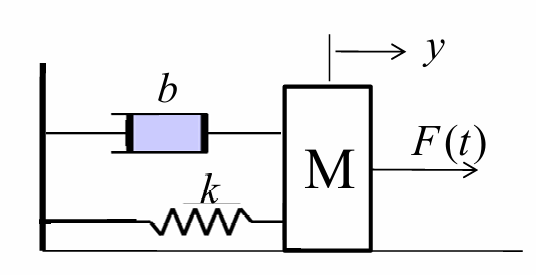
\includegraphics[width=0.3\textwidth]{note/mathmodel/figure/1.png}
    \end{center}

    \begin{equation*}
        \begin{split}
            &M\ddot{y} + ky + b\dot{y} = F(t) \\
            &M\dot{v} + bv + k \int_0^t v(\tau) d\tau = F(t)\\
        \end{split}
    \end{equation*}
\end{example}

\begin{example}
    如图所示为RLC并联电路，设外界输入为$I(t)$ ，电路中输出量为：$i_L$ 和$u_c$ ，则可以列出以下式子：
    \begin{center}
        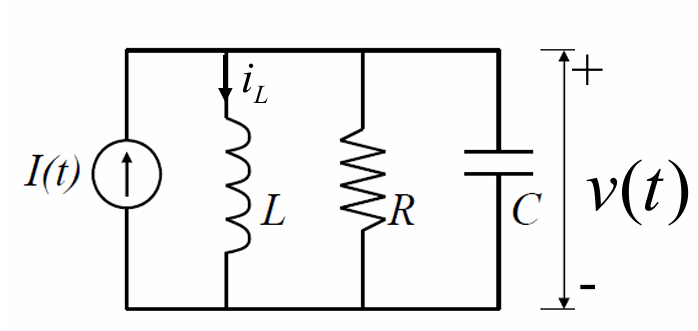
\includegraphics[width = .3\textwidth]{note/mathmodel/figure/2.png}
    \end{center}

    \begin{equation*}
        \begin{split}
            &C\dot{u_c} + \frac{1}{R}u_c + \frac{1}{L} \int_0^t u_c(\tau) d\tau = I(t) \\
            &CL\ddot{i_L} +\frac{L}{R}\dot{i_L} + i_L = I(t) 
        \end{split}
    \end{equation*}

\end{example}

\section{Laplace变换}
\begin{definition}[拉氏变换]
    Laplace变换可以简略定义为如下形式：
    \begin{equation*}
        F(s) = \mathcal{L}[f(t)] = \int_{0^{-}}^\infty f(t) e^{-st} dt 
    \end{equation*}
    当且仅当$f(t) e^{-st}$ 绝对可积 \\
    当然，在物理中可实现信号通常都是可变换的
\end{definition}

\begin{definition}[拉氏逆变换]
    Laplace逆变换可以简略定义为如下形式：
    \begin{equation*}
        f(t) = \mathcal{L}^{-1} [F(s)] = \frac{1}{2\pi j} \int_{\sigma - j \infty} ^{\sigma + j\infty} F(s) e^{st} dt
    \end{equation*}
    当我们掌握留数的知识后，Laplace逆变换可以用下述式子计算：\\
    设$F(s)$ 的极点为：$s_1,s_2,\cdots,s_n$，则：
    \begin{equation*}
        f(t) = \mathcal{L}^{-1} [F(s)] = \Sigma_{i=1}^n Res[F(s)e^{st},s_i]
    \end{equation*}
\end{definition}

\begin{property}[Laplace变换的性质]
    \begin{enumerate}
        \item 线性性：$\Lcal [\alpha f_1(t) + \beta f_2(t)] = \alpha \Lcal[f_1(t)] + \beta \Lcal[f_2(t)] $ 
        \item 时移性：$\Lcal [f(t-\lambda)] = e^{-s\lambda} \Lcal [f(t)]$ 
        \item 时域伸缩性：$\Lcal [f(at)] = \dfrac{1}{a} \Lcal[f(t)](\dfrac{s}{a}) $
        \item 频移性：$\Lcal[e^{-at}f(t)] = \Lcal[f(t)] (s+a)$ 
        \item 微分性：$\Lcal[\dfrac{d}{dt}f(t)] = s\Lcal[f(t)] - f(0^-)$ 
        \item 积分性：$\Lcal [\int_0^t f(\xi) d\xi] = \dfrac{\Lcal[f(t)]}{s}$ 
        \item 时域卷积：$\Lcal [f_1 * f_2] = \Lcal[f_1]\cdot \Lcal[f_2]$ 
        \item 频域卷积：$\Lcal [f_1\cdot f_2]= \dfrac{1}{2\pi j} \Lcal[f_1] * \Lcal[f_2]$
        \item 频域微分：$\Lcal [tf(t)] = -\dfrac{d}{ds}\Lcal[f(t)] $
        \item 初值定理：$\lim_{t\rightarrow 0^+} f(t) = \lim _{s\rightarrow \infty} s\Lcal[f(t)]$
        \item 终值定理：$ \lim_{t\rightarrow \infty} f(t) = \lim_{s\rightarrow 0} s\Lcal[f(t)]$
    \end{enumerate}
\end{property}

\section{传递函数}
\begin{definition}[传递函数]
    在零初始条件下，线性定常系统或元件输出信号的Laplace变换式$Y(s)$与输入信号的Laplace变换式$R(s)$之比为该系统或元件的传递函数。数学表示为：
    \begin{equation*}
        G(s) = \frac{Y(s)}{R(s)} = \frac{b_m s^m + b_{m-1} s^{m-1} + \cdots + b_1 s +b_0}{s^n + a_{n-1} s^{n-1}+\cdots + a_1 s +a_0}
    \end{equation*}
    注：
    \begin{itemize}
        \item 传递函数反映系统零状态响应的传递关系
        \item 传递函数表明了系统数学模型的阶次n，它表征着系统的固有特性（如系统的结构与参数等），与输入的形式无关
        \item 传递函数是研究线性系统动态特性的重要工具
    \end{itemize}

\end{definition}


\subsection{典型环节的传递函数}
\begin{enumerate}
    \item 惯性环节：$G(s) = \dfrac{1}{Ts+1}$ ，$T$为时间常数
    \item 积分环节：$G(s) = \dfrac{1}{Ts}$ ， $T$为时间常数
    \item 震荡环节：$G(s) = \dfrac{\omega_n^2}{s^2 + 2\zeta \omega_n s + \omega_n^2}$ ，$\zeta$ 为阻尼比，$\omega_n$ 为无阻尼自然震荡角频率
    \item 微分环节：$G(s) = T_d s$
    \item 比例环节：$G(s) = K_p$
    \item 时滞/延迟环节：$G(s) = e^{-\tau s}$ 
\end{enumerate}

\subsection{系统方框图模型}
\begin{definition}[方框图]
    系统方框图模型是系统各环节的传递函数功能和信号流向的图解表示，是一种图形化的数学模型，如下图所示：
    \begin{center}
        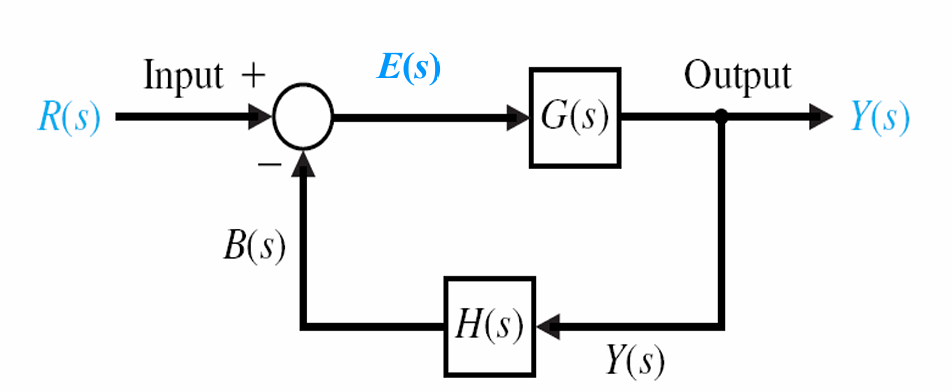
\includegraphics[width=.3\textwidth]{note/mathmodel/figure/3.png}
    \end{center}
    此图为负反馈控制系统的典型结构图，包含以下三个重要参数：
    \begin{enumerate}
        \item 闭环传递函数：$\dfrac{Y(s)}{R(s)}$
        \item 前向传递函数：$\dfrac{Y(s)}{E(s)}$
        \item 开环传递函数：$\dfrac{B(s)}{E(s)}$
    \end{enumerate}
    同时也包含四种基本单元：
    \begin{enumerate}
        \item 信号线
        \item 分支点（引出点、测量点）
        \item 相加点（比较点，综合点）
        \item 方框
    \end{enumerate}
    示例图如下所示：
    \begin{center}
        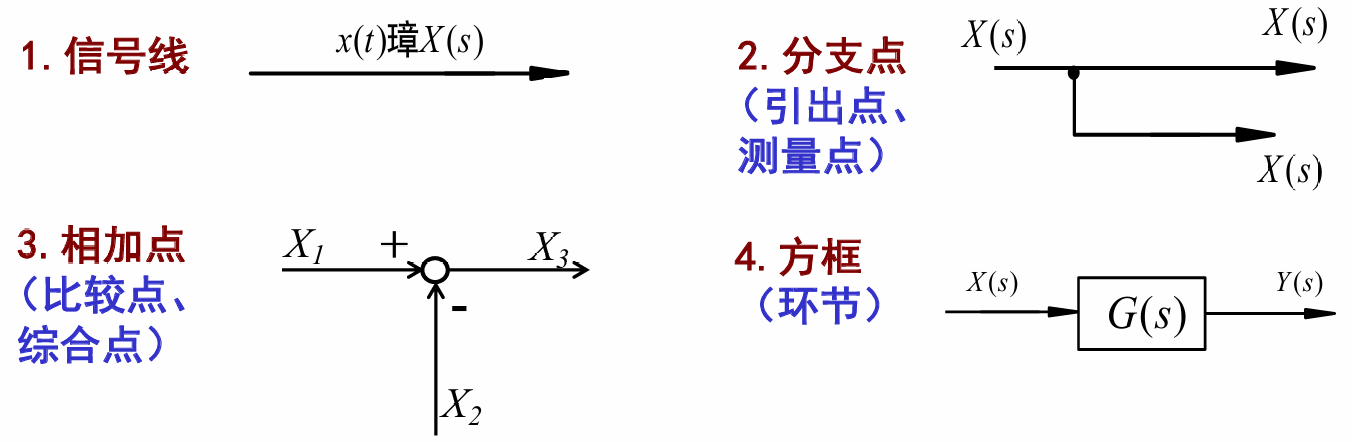
\includegraphics[width = .4\textwidth]{note/mathmodel/figure/4.png}
    \end{center}
\end{definition}

\begin{ascolorbox5}{框图的基本变换}[black!50!white][coltext = black]
    \begin{enumerate}
        \item 合并串联方框：
        \begin{center}
            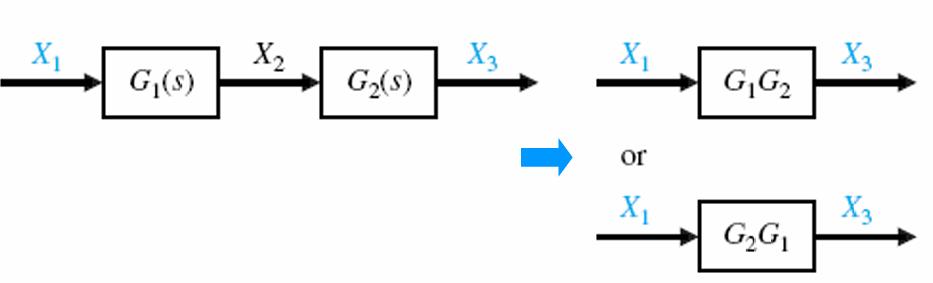
\includegraphics[width = .4\textwidth]{note/mathmodel/figure/5.png}
        \end{center}
        \item 相加点后移：
        \begin{center}
            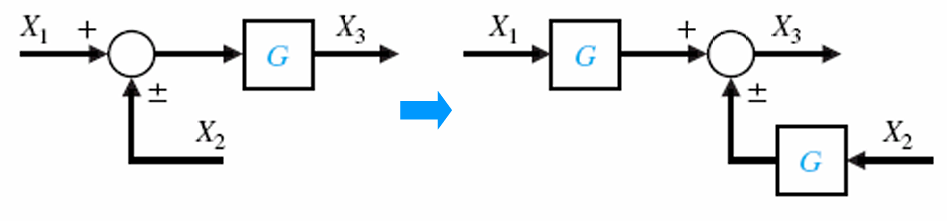
\includegraphics[width = .4\textwidth]{note/mathmodel/figure/6.png}
        \end{center}
        \item 相加点前移：
        \begin{center}
            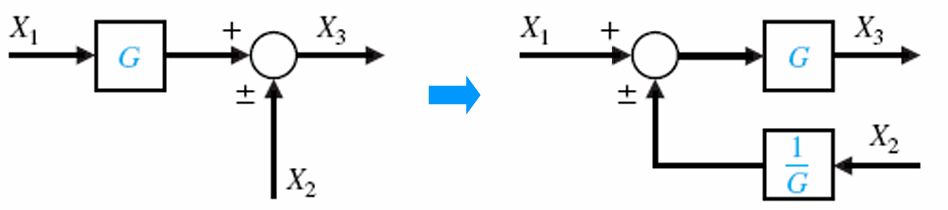
\includegraphics[width = .4\textwidth]{note/mathmodel/figure/7.png}
        \end{center}
        \item 分支点后移：
        \begin{center}
            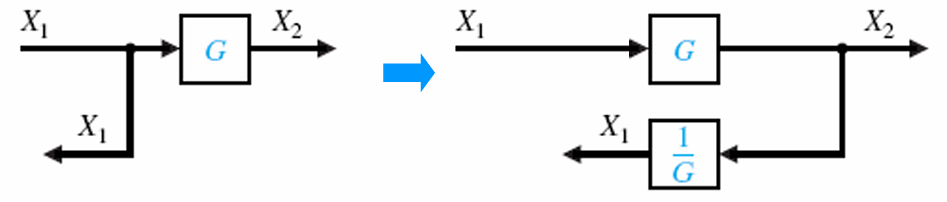
\includegraphics[width = .4\textwidth]{note/mathmodel/figure/8.png}
        \end{center}
        \item 分支点前移：
        \begin{center}
            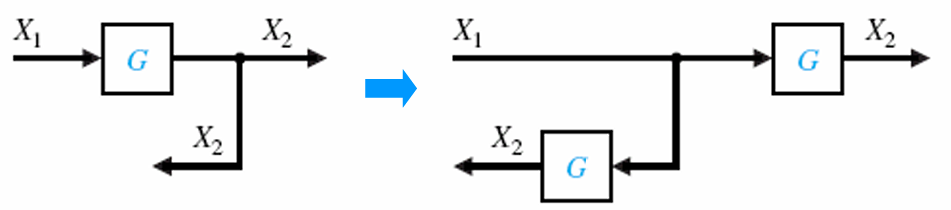
\includegraphics[width = .4\textwidth]{note/mathmodel/figure/9.png}
        \end{center}
        \item 消去反馈通路：
        \begin{center}
            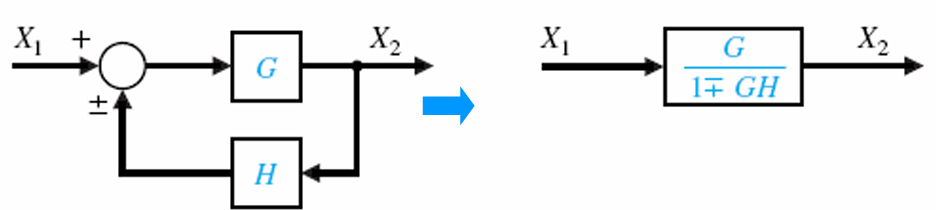
\includegraphics[width = .4\textwidth]{note/mathmodel/figure/10.png}
        \end{center}
        \item 并联方框：
        \begin{center}
            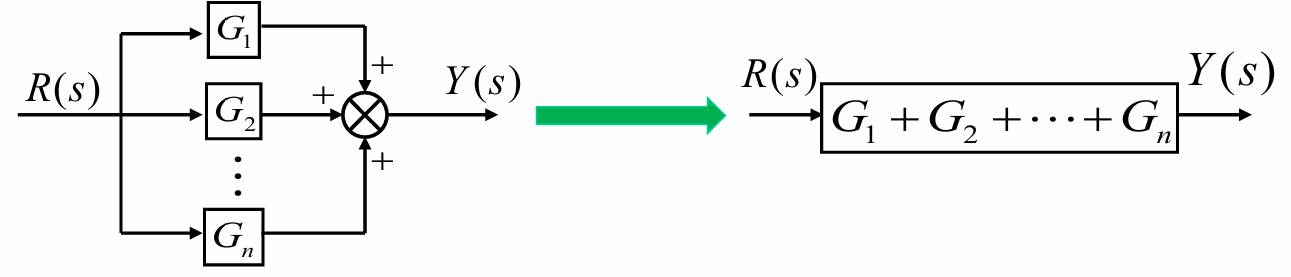
\includegraphics[width = .5\textwidth]{note/mathmodel/figure/11.png}
        \end{center}
        \item 相邻相加点之间的移动：
        \begin{center}
            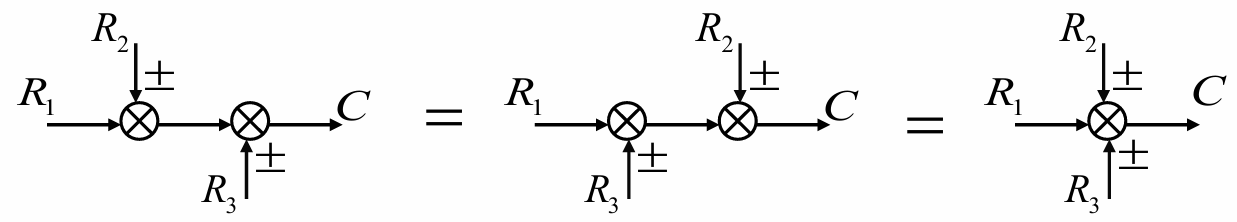
\includegraphics[width = .5\textwidth]{note/mathmodel/figure/12.png}
        \end{center}
        \item 相加点与分支点交换位置：
        \begin{center}
            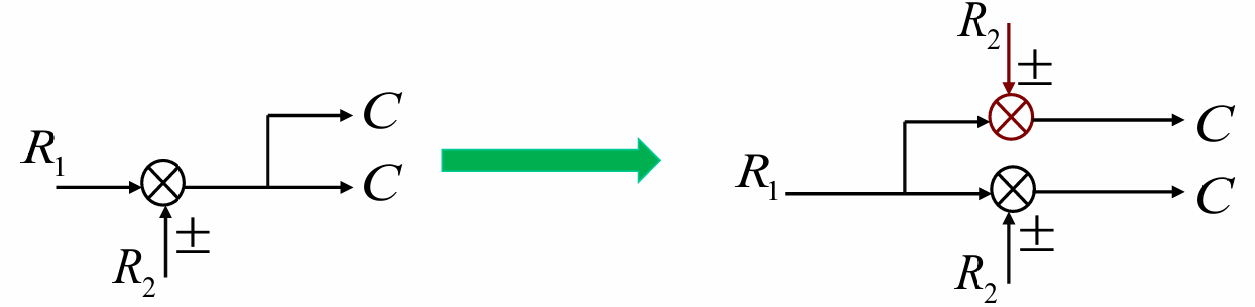
\includegraphics[width = .5\textwidth]{note/mathmodel/figure/13.png}
        \end{center}
    \end{enumerate}
\end{ascolorbox5}

\begin{example}
    化简以下方框图：
    \begin{center}
        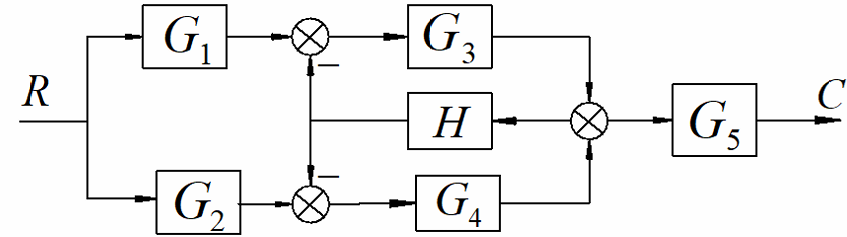
\includegraphics[width = .4\textwidth]{note/mathmodel/figure/14.png}
    \end{center}
    解答如下：
    \begin{itemize}
        \item[(1)] 相加点后移：
        \begin{center}
            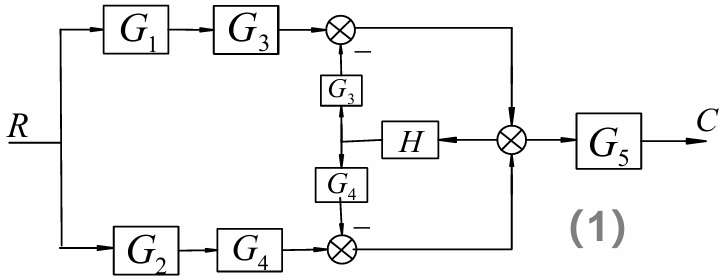
\includegraphics[width = .4\textwidth]{note/mathmodel/figure/15.png}
        \end{center}
        \item[(2)] 分支点前移：
        \begin{center}
            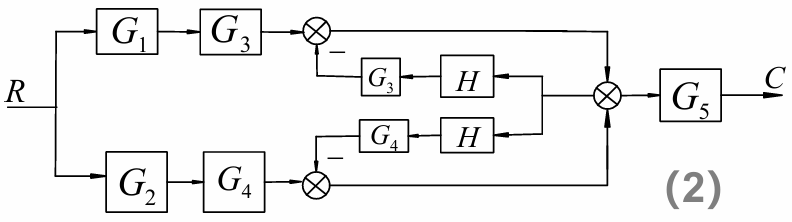
\includegraphics[width = .4\textwidth]{note/mathmodel/figure/16.png}
        \end{center}
        \item[(3)] 合并串联部分：
        \begin{center}
            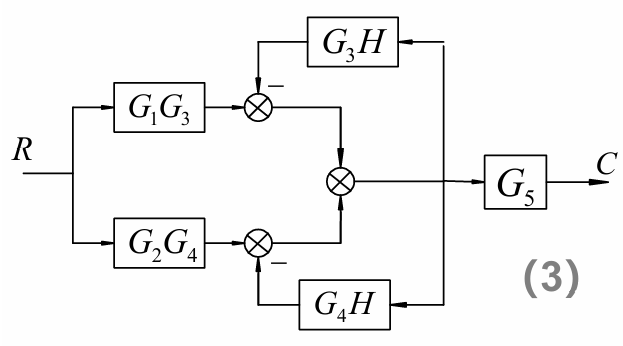
\includegraphics[width = .3\textwidth]{note/mathmodel/figure/17.png}
        \end{center}
        \item[(4)] 拆分相加点：
        \begin{center}
            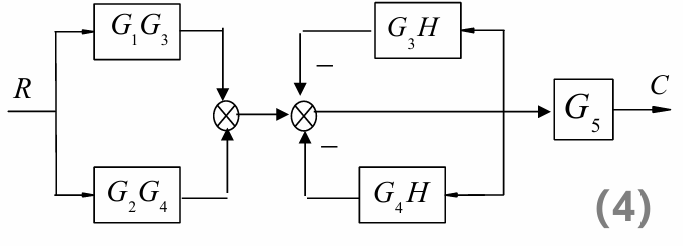
\includegraphics[width = .4\textwidth]{note/mathmodel/figure/18.png}
        \end{center}
        \item[(5)] 合并并联和反馈部分：
        \begin{center}
            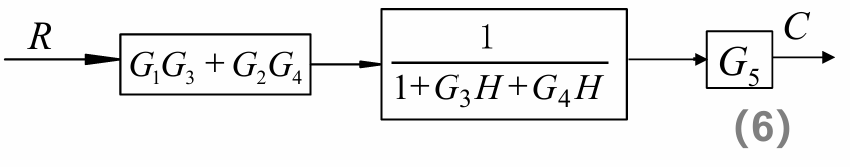
\includegraphics[width = .4\textwidth]{note/mathmodel/figure/19.png}
        \end{center}
        \item[(6)] 合并串联部分：
        \begin{center}
            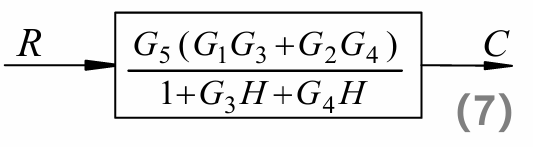
\includegraphics[width = .3\textwidth]{note/mathmodel/figure/20.png}
        \end{center}
    \end{itemize}
\end{example}

\subsection{信号流图}

\begin{definition}[信号流图]
    信号流图是用来表示系统中各变量间相互关系以及信号传递的一种图解方法，包含以下几个部分：
    \begin{enumerate}
        \item 节点（node）：表示系统的变量，用$\circ$表示
        \item 支路（branch）：相当于乘法器，信号流经支路时，被乘以支路增益而变换为另一信号
    \end{enumerate}
    注：
    \begin{itemize}
        \item 信号在支路上只能沿箭头单向传递
        \item 节点具有以下作用：
        \begin{enumerate}
            \item 对所有来自流入支路信号作加法运算
            \item 将流入信号之和传输给所有流出支路
        \end{enumerate}
    \end{itemize}
    一些有关的术语：
    \begin{itemize}
        \item 输入节点（源点）：输入信号对应的节点。只有输出支路，无输入支路
        \item 输出节点（阱点）：输出信号对应的节点，常用传输为1的支路引出。只有输入，没有输出支路
        \item 混合节点：既有输出支路，又有输入支路
        \item 前向通路：当信号从输入节点至输出节点传递时，每个节点只通过一次的通路
        \item 回路：起点和重点是同一节点，而且信号通过每个节点不多于1次的闭合通路
        \item 不接触回路：之间没有公共节点的回路
    \end{itemize}
\end{definition}

\begin{ascolorbox1}{信号流图与方框图之间的转化}[]
    如下图所示为信号流图与方框图之间的转化表：
    \begin{center}
        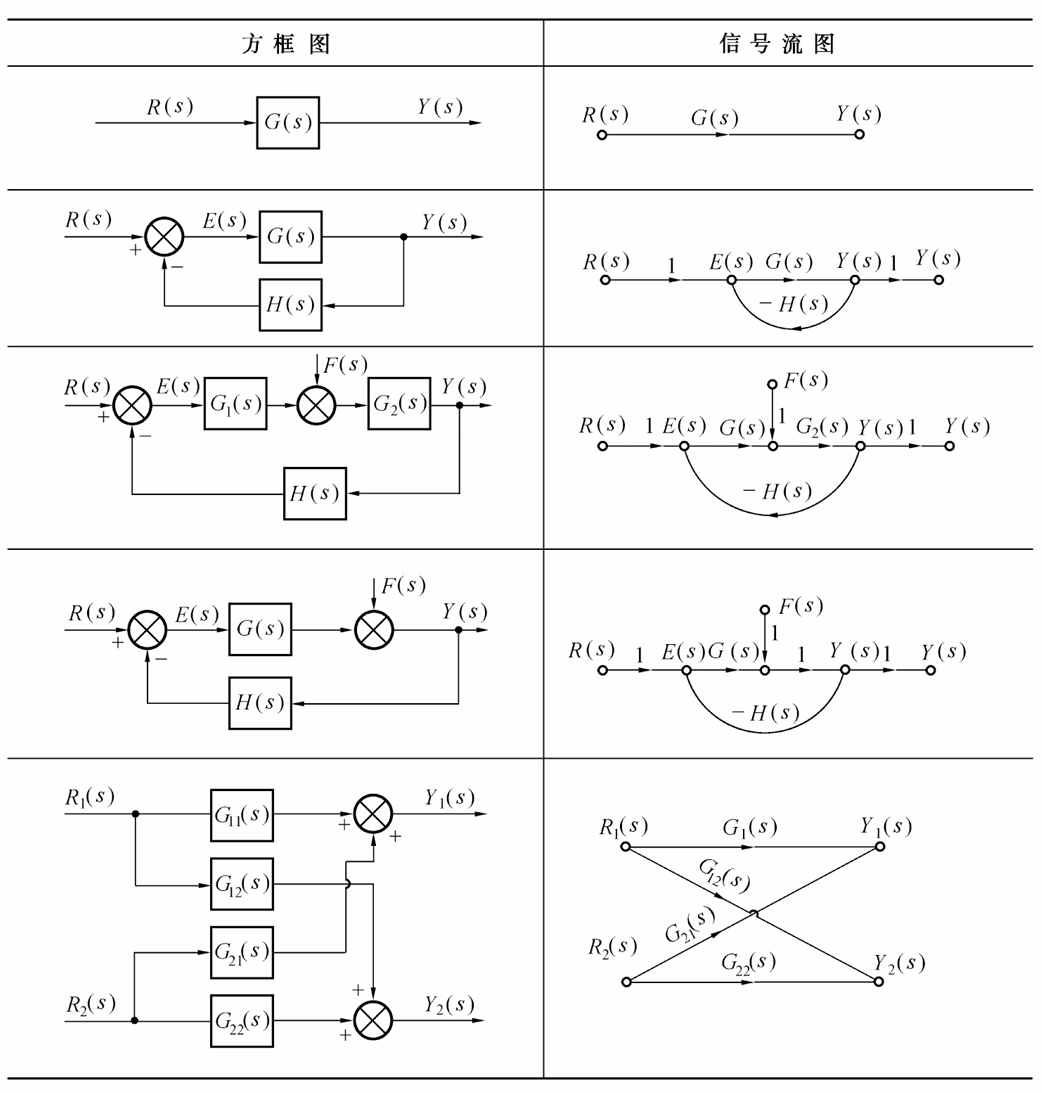
\includegraphics[width = .5\textwidth]{note/mathmodel/figure/21.png}
    \end{center}
\end{ascolorbox1}

\subsection{梅森公式(Mason's formula)}

\begin{definition}
    Mason 公式由以下数学式子给出：
    \begin{equation*}
        P = \frac{1}{\Delta} \Sigma_{k=1}^n P_k \Delta_k
    \end{equation*}
    其中：
    \begin{itemize}
        \item $P$ ：总增益
        \item $P_k$：第k条前向通路的通路增益
        \item $\Delta = 1-\Sigma_{l_1} L_1 + \Sigma_{l_1 l_2} L_1 L_2 -\Sigma_{l_1 l_2 l_3} L_1 L_2 L_3 \cdots +(-1)^n \Sigma_{l_1 l_2 \cdots l_n} L_1 L_2 \cdots L_n \cdots$ 为系统结构图的特征式
        \item $\Sigma_{l_1 l_2 \cdots l_k} L_1 L_2 \cdots L_k$ 为每k个互不接触回路增益乘积之和 ($1\leq k \leq$ 最大回路数)
        \item $\Delta_k$：在特征式中除去与第k条前向通路相接触的回路后的特征式，称为第k条前向通路特征式的余子式
    \end{itemize}
\end{definition}

\begin{example}
    用Mason 增益公式求出以下系统方框图中的传递函数：
    \begin{center}
        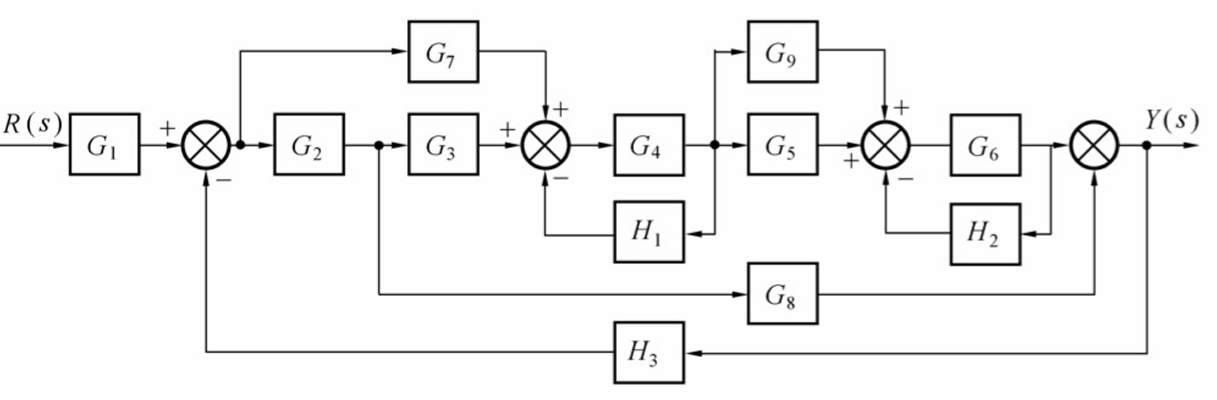
\includegraphics[width=.5\textwidth]{note/mathmodel/figure/22.png}
    \end{center}
    解答如下：
    \begin{itemize}
        \item[(1)] 图中回路增益分别为：
        \begin{equation*}
            \begin{split}
                L_1 = &-G_4 H_1 \\
                L_2 = &-G_6 H_2 \\
                L_3 = &-G_2 G_3 G_4 G_5 G_6 H_3 \\
                L_4 = &-G_2 G_3 G_4 G_9 G_6 H_3 \\
                L_5 = & -G_7 G_4 G_5 G_6 H_3 \\
                L_6 = & -G_7 G_4 G_9 G_6 H_3 \\
                L_7 = & -G_2 G_8 H_3 \\
            \end{split}
        \end{equation*}
        \item[(2)] 每两个互不接触回路增益乘积：
        \begin{equation*}
            \begin{split}
                L_1 L_2 = &G_4 G_6 H_1 H_2 \\
                L_1 L_7 = & G_2 G_4 G_8 H_1 H_3 \\
                L_2 L_7 = & G_2 G_6 G_8 H_2 H_3 \\
            \end{split}
        \end{equation*}
        \item[(3)] 每三个互不接触回路乘积：
        \begin{equation*}
            L_1 L_2 L_7 = -G_2 G_4 G_6 G_8 H_1 H_2 H_3
        \end{equation*}
        \item[(4)] 方框图特征式：
        \begin{equation*}
            \begin{split}
                \Delta =& 1-\Sigma_{i=1}^7 L_i +L_1 L_2 +L_1 L_7 +L_2 L_7-L_1 L_2 L_7\\
                =& 1+G_4 H_1+G_6 H_2+G_2 G_3 G_4 G_5 G_6 H_3+G_2 G_3 G_4 G_9 G_6 H_3+G_7 G_4 G_5 G_6 H_3+G_7 G_4 G_9 G_6 H_3+G_2 G_8 H_3 \\
                &+G_4 G_6 H_1 H_2+G_2 G_4 G_8 H_1 H_3+G_2 G_6 G_8 H_2 H_3
            \end{split}
        \end{equation*}
        \item[(5)] 前向通路增益及其余子式：
        \begin{equation*}
            \begin{split}
                P_1 = G_1 G_2 G_3 G_4 G_5 G_6 \quad &\Delta_1 = 1 \\
                P_2 = G_1 G_2 G_8 \quad &\Delta_2 = 1 + G_4 H_1 + G_6 H_2 +G_4 G_6 H_1 H_2 \\
                P_3 = G_1 G_7 G_4 G_5 G_6 \quad & \Delta_3 = 1 \\
                P_4 = G_1 G_2 G_3 G_4 G_9 G_6 \quad &\Delta_4 = 1 \\
                P_5 = G_1 G_7 G_4 G_9 G_6 \quad &\Delta_5 = 1 \\
            \end{split}
        \end{equation*}
        \item[(6)] 由Mason 增益公式$P = \dfrac{1}{\Delta} \Sigma_{k=1}^3 P_k \Delta_k$ 即可得出答案（答案过长不方便写在此处）
    \end{itemize}
\end{example}

